\section{Experimental}
\subsection{Hardware \& Software}
\subsubsection{Hardware}
A variety of hardware and computers where used to perform the tests, however below is an example of what was used:
\begin{itemize}
    \item CPU: AMD Ryzen 5600x
    \item GPU: AMD Radeon RX 6650 XT
    \item RAM: 16gb
\end{itemize}
\subsubsection{Software}
\begin{itemize}
    \item Operating System: Windows 11
    \item Programming Language: Python 3.12.6
    \item External Libraries used:
    \begin{itemize}
        \item[•] pandas==2.2.3
        \item[•] plotly==5.24.1
        \item[•] matplotlib==3.9.2
        \item[•] seaborn==0.13.2
        \item[•] marimo==0.8.19
        \item[•] numpy==2.1.1
        \item[•] scipy==1.14.1
    \end{itemize}
    \item Standard Libraries used:
    \begin{itemize}
        \item[•] ast
        \item[•] time
        \item[•] logging
    \end{itemize}
    \item Development Enviroment:
    \begin{itemize}
        \item[•] Visual studio code
        \item[•] Jupiter Notebooks
        \item[•] Marimo
        \item[•] Github
    \end{itemize}
    \item Version Control:
    \begin{itemize}
        \item[•] Git
    \end{itemize}
\end{itemize}
\subsection{Procedure}
\subsubsection{Initial setup}
Initial setup inform of having different strategies and parameters to benchmark against each other, as well as having a way of visualizing everything \& a way of representing the solution.
\subsubsection{Representation of solution}
Example of a solution below:
\begin{verbatim}
    [6 3 5 8 1 4 2 7]
\end{verbatim}
Solutions are being represented as a python list where the index of the integer is the column and the value of the integer is the row. That means the first element 6 would be equivalent to A6 on a chessboard. We evaluate the fitness of a solution the following way:
\begin{equation}
    \frac{\text{\#}\; \text{Conflicts}}{\text{Denominator}}
\end{equation}
The denominator being the maximum number of ways to choose 2 queens from N to create a conflict is given by:
\begin{equation}
    \binom{N}{2} = \frac{N(N-1)}{2}
\end{equation}
\begin{verbatim}
    For N = 8 We would get:
\end{verbatim}
\begin{equation}
    \frac{\text{\#}\; \text{Conflicts}}{28}
\end{equation}
\subsubsection{Strategies}
A variety of strategies where implemented, the recombinatorial ones being:
\begin{itemize}
    \item even cut and crossfill
    \item one cut crossover
    \item two cut crossover
    \item partially mapped crossover
    \item pmx dp rm (remember to check)
    \item ordered crossover
\end{itemize}
Mutation ones:
\begin{itemize}
    \item swap mutation
    \item inversion mutation
    \item duplicate replacement
    \item creep mutation
    \item scramble mutation
\end{itemize}
Initialization strategies:
\begin{itemize}
    \item completely random
    \item random permutations
\end{itemize}
Parent selection strategy:
\begin{itemize}
    \item Tournament selection
\end{itemize}
Survival selection strategies:
\begin{itemize}
    \item prob survival (select by fitness)
    \item del rep 2 (replace by offspring)
\end{itemize}
Genocide strategies:
\begin{itemize}
    \item static stagnation
    \item dynamic stagnation
\end{itemize}
\subsubsection{Parameters}
\begin{itemize}
    \item Population size
    \item Number of offspring rate
    \item Recombination rate
    \item Mutation rate
    \item Tournament group size
    \item Iterations
    \item Max evaluations
\end{itemize}
\subsubsection{Early tests}
Early on we focused on modularizing everything in order to be able to easily swap and implement new strategies, this part was crucial for our testing. The early tests where rather limited compared to the later ones, we just implemented new ideas and tested them against each other but there wasn't really a way to quantify whether something was better than the other, other than watching the evaluations being printed into the terminal.
\subsubsection{Finding the best setup}
Firstly a definition of "best" was needed, we decided on counting the evaluations needed to find a solution. The idea was to create a bunch of permutations of the strategies and parameters and then run them for a larger amount of iterations then dividing the evaluations per strategy by the iterations, for clarifying sake:
\begin{equation}
\frac{\text{Total}\; \text{Evaluations}}{\text{Iterations}}
\end{equation}
We created our own module named
\begin{verbatim}
    parameter_tuning.py
\end{verbatim}
In which we use Latin Hypercube Sampling in order to tune our parameters and choose a random strategies from our list of strategies mentioned above. We then visualize everything using bar-chart, see:
\begin{verbatim}
    visuals.py -> def strategy_plot():
\end{verbatim}
We have another parameter called topX in which you can specify a number X of the top performing setups to extract into a file fittingly called:
\begin{verbatim}
    topX_setups.py
\end{verbatim}
Since running a lot of setups for a larger number of iterations can take time we used threading in order to speed up the entire experimental process. if you are interested in seeing how we implemented threading please see:
\begin{verbatim}
    put file name here .py
\end{verbatim}
there where some patterns already here, for instance things like pmx\_dp\_rm (partially mapped crossover duplicate removal) \& duplicate removal mutation where among the things that kept showing up. Thinking about these results logically, it puts us on a better evaluation instantly if we eliminate duplicates since that would mean queens are on the same row if their indexes are identical.
\\\\
However to confirm our beliefs we decided to isolate strategies and parameters, meaning we statically assigned some and the ones we wanted to explore as dynamic.
\\\\
We started experimenting with genocide, and found that a genetic algorithm with genocide performs substantially better than one without. One can through dynamic methods adjust the functionality of the genetic algorithm so that it performs better for some specified genome sizes of interest.
\subsubsection{The data}

The image below might be hard to view so please zoom in.
\\~\\
\begin{figure}[ht]
\centering
\makebox[\linewidth]{%
  \setlength\fboxsep{1pt}%<- optional for padding
  \colorbox{black}{%
    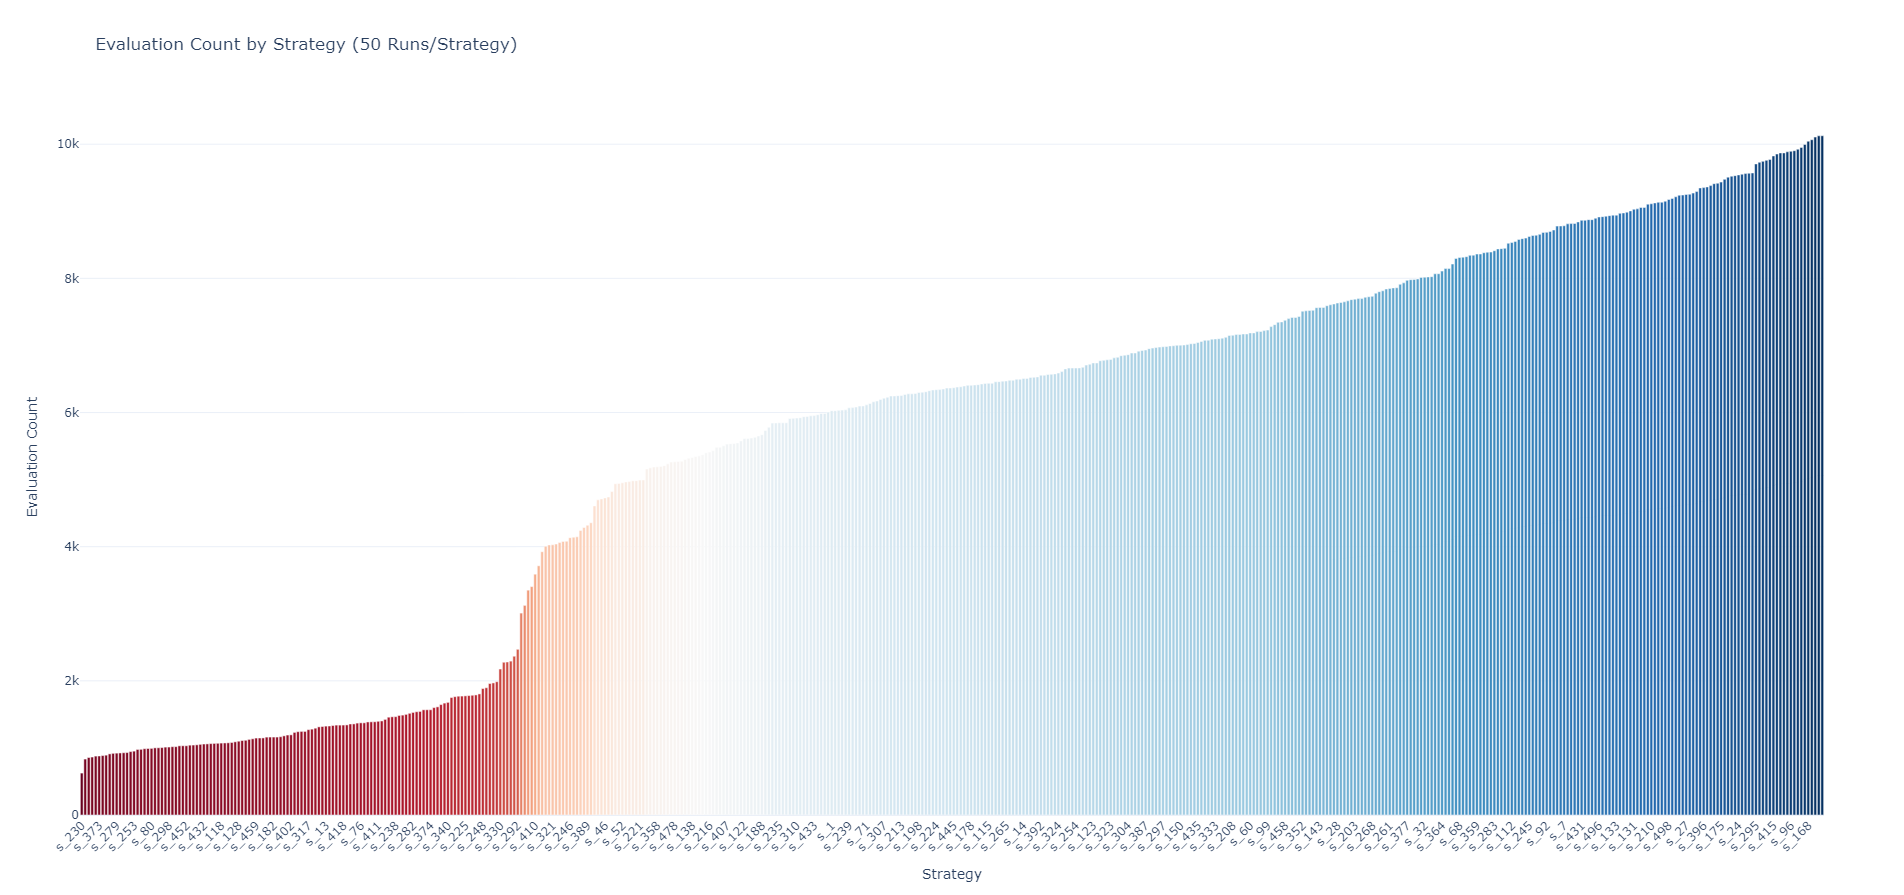
\includegraphics[width=1.5\textwidth]{img/50x500 new.png}}}
    \caption{Plot of the different setups generated, with randomized strategies and parameters}
\end{figure}
\\
The plot above generated shows how the different setups compare to each other, in order to not make a huge list below setup\_38 has been extracted, which was the top performing one:
\\
\begin{verbatim}
    s_38 = {
            'GENOME_SIZE': 8,
            'POPULATION_SIZE': 200,
            'NUM_OFFSPRING_RATE': 0.4,
            'TOURNAMENT_GROUP_SIZE': 0.45,
            'MAX_FITNESS_EVALUATIONS': 10000,
            'fitness_strategy': 'conflict_based',
            'termination_strategy': 'evaluation_count',
            'visualization_strategy': 'terminal',
            'metric_strategy': 'avg_similarity',
            'logging_strategy': 'logger',
            'print_type': 'csv_file',
            'POPULATION_SIZE': 189,
            'NUM_OFFSPRING_RATE': 0.423,
            'RECOMBINATION_RATE': 0.741,
            'MUTATION_RATE': 0.079,
            'TOURNAMENT_GROUP_SIZE': 0.364,
            'initialization_strategy': 'random',
            'parent_selection_strategy': 'tournament',
            'recombination_strategy': 'pmx_dp_rm',
            'mutation_strategy': 'duplicate_replacement',
            'survival_selection_strategy': 'prob_survival',
        }
\end{verbatim}
The problem with analysing the strategies and parameters like this, is that we aren't isolating them everything gets randomized and put into a setup.
\\\\
Below is a plot of some setup, the parameters and strategies for this one are irrelevant; With a genome size of 7 were we are comparing the algorithm with and without genocide
\begin{figure}[ht]
\centering
\makebox[\linewidth]{%
  \setlength\fboxsep{1pt}%<- optional for padding
  \colorbox{black}{%
    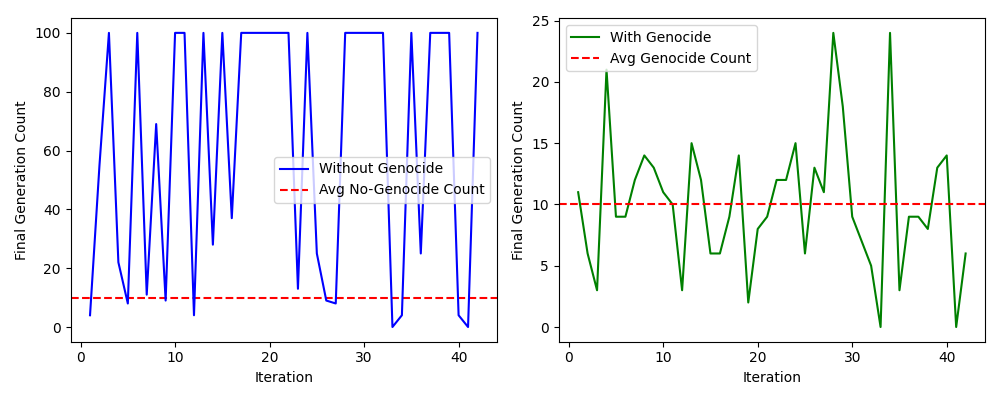
\includegraphics[width=1.5\textwidth]{img/Genome size 7, With and without genocide.png}}}
    \caption{Genome size 7, without and with genocide}
\end{figure}
\\\\
As you can see running the algorithm with genocide provides a higher average.